% ***************************************************
% Appendix
% ***************************************************
\chapter{Appendix}

Write your appendix here. Following two are examples. 


\section{Neorv32 memory address space layout}
\label{app:mem_address}
\begin{figure}[h!]
    \centering
    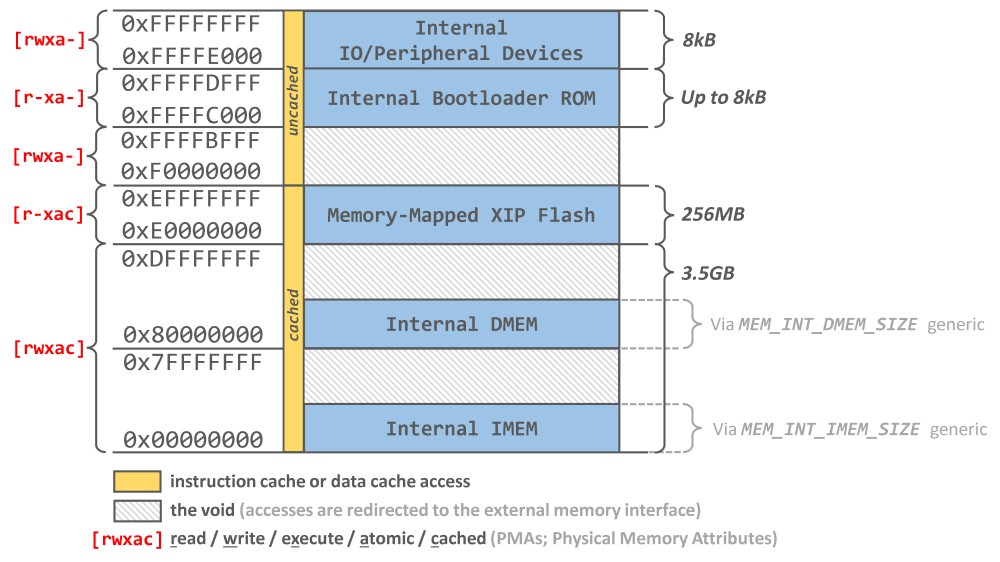
\includegraphics[width=1\textwidth]{Images/neorv32_address_space.png}
    \caption{Neorv32 Memory Address space.}
\end{figure}



\section{FPGA primitives utilisation}
\label{app:res_usage}
\begin{table}
    \centering
    \caption{FPGA primitives utilisation for XC7A100T}
    \begin{tabular}{|l|r|l|}
        \toprule
        Ref Name   & Used & Functional Category \\
        \midrule
        LUT6       & 16262 & LUT \\
        LUT5       & 14820 & LUT \\
        FDRE       & 14500 & Flop \& Latch \\
        LUT3       & 13222 & LUT \\
        MUXF7      &  2436 & MuxFx \\
        FDCE       &  1875 & Flop \& Latch \\
        RAMD64E    &  1836 & Distributed Memory \\
        LUT4       &  1294 & LUT \\
        LUT2       &  1016 & LUT \\
        MUXF8      &   884 & MuxFx \\
        CARRY4     &   437 & CarryLogic \\
        LUT1       &   156 & LUT \\
        RAMB36E1   &   130 & Block Memory \\
        FDPE       &    41 & Flop \& Latch \\
        OBUF       &    40 & IO \\
        LDCE       &    36 & Flop \& Latch \\
        IBUF       &    24 & IO \\
        SRLC32E    &    21 & Distributed Memory \\
        OBUFT      &    11 & IO \\
        BUFG       &     8 & Clock \\
        FDSE       &     5 & Flop \& Latch \\
        DSP48E1    &     4 & Block Arithmetic \\
        SRL16E     &     1 & Distributed Memory \\
        MMCME2\_ADV &    1 & Clock \\
        \bottomrule
    \end{tabular}
\end{table}

\begin{table}
    \centering
    \caption{Memory Utilisation}
    \begin{tabular}{|l|r|r|r|r|r|}
        \toprule
        Site Type      & Used & Fixed & Prohibited & Available & Util\% \\
        \midrule
        Block RAM Tile &  130 &     0 &          0 &       135 & 96.30 \\
        RAMB36/FIFO*   &  130 &     0 &          0 &       135 & 96.30 \\
        RAMB36E1 only  &  130 &     - &          - &         - &    -  \\
        RAMB18         &    0 &     0 &          0 &       270 &  0.00 \\
        \bottomrule
    \end{tabular}
\end{table}

\begin{table}
    \centering
    \caption{Slice Logic Utilisation}
    \begin{tabular}{|l|r|r|r|r|r|}
        \toprule
        Site Type                 & Used & Fixed & Prohibited & Available & Util\% \\
        \midrule
        Slice LUTs*               & 40920 &     0 &          0 &     63400 & 64.54 \\
        LUT as Logic              & 39062 &     0 &          0 &     63400 & 61.61 \\
        LUT as Memory             &  1858 &     0 &          0 &     19000 &  9.78 \\
        LUT as Distributed RAM    &  1836 &     - &          - &         - &    -  \\
        LUT as Shift Register     &    22 &     - &          - &         - &    -  \\
        Slice Registers           & 16457 &     0 &          0 &    126800 & 12.98 \\
        Register as Flip Flop     & 16421 &     0 &          0 &    126800 & 12.95 \\
        Register as Latch         &    36 &     0 &          0 &    126800 &  0.03 \\
        F7 Muxes                  &  2436 &     0 &          0 &     31700 &  7.68 \\
        F8 Muxes                  &   884 &     0 &          0 &     15850 &  5.58 \\
        \bottomrule
    \end{tabular}
\end{table}
